% !Mode:: "TeX:UTF-8"
\chapter{视觉里程计2}
\label{cpt:vo2}
\begin{mdframed}  
	\textbf{主要目标}
	\begin{enumerate}[labelindent=0em,leftmargin=1.5em]
		\item 理解光流法跟踪特征点的原理。
		\item 理解直接法是如何估计相机位姿的。
		\item 实现多层直接法的计算。
	\end{enumerate}
\end{mdframed}

直接法是视觉里程计另一主要分支,它与特征点法有很大不同。虽然它还没有成为现在VO中的主流,但经过近几年的发展,直接法在一定程度上已经能和特征点法平分秋色。本讲我们将介绍直接法的原理,并实现直接法中的核心部分。

\newpage
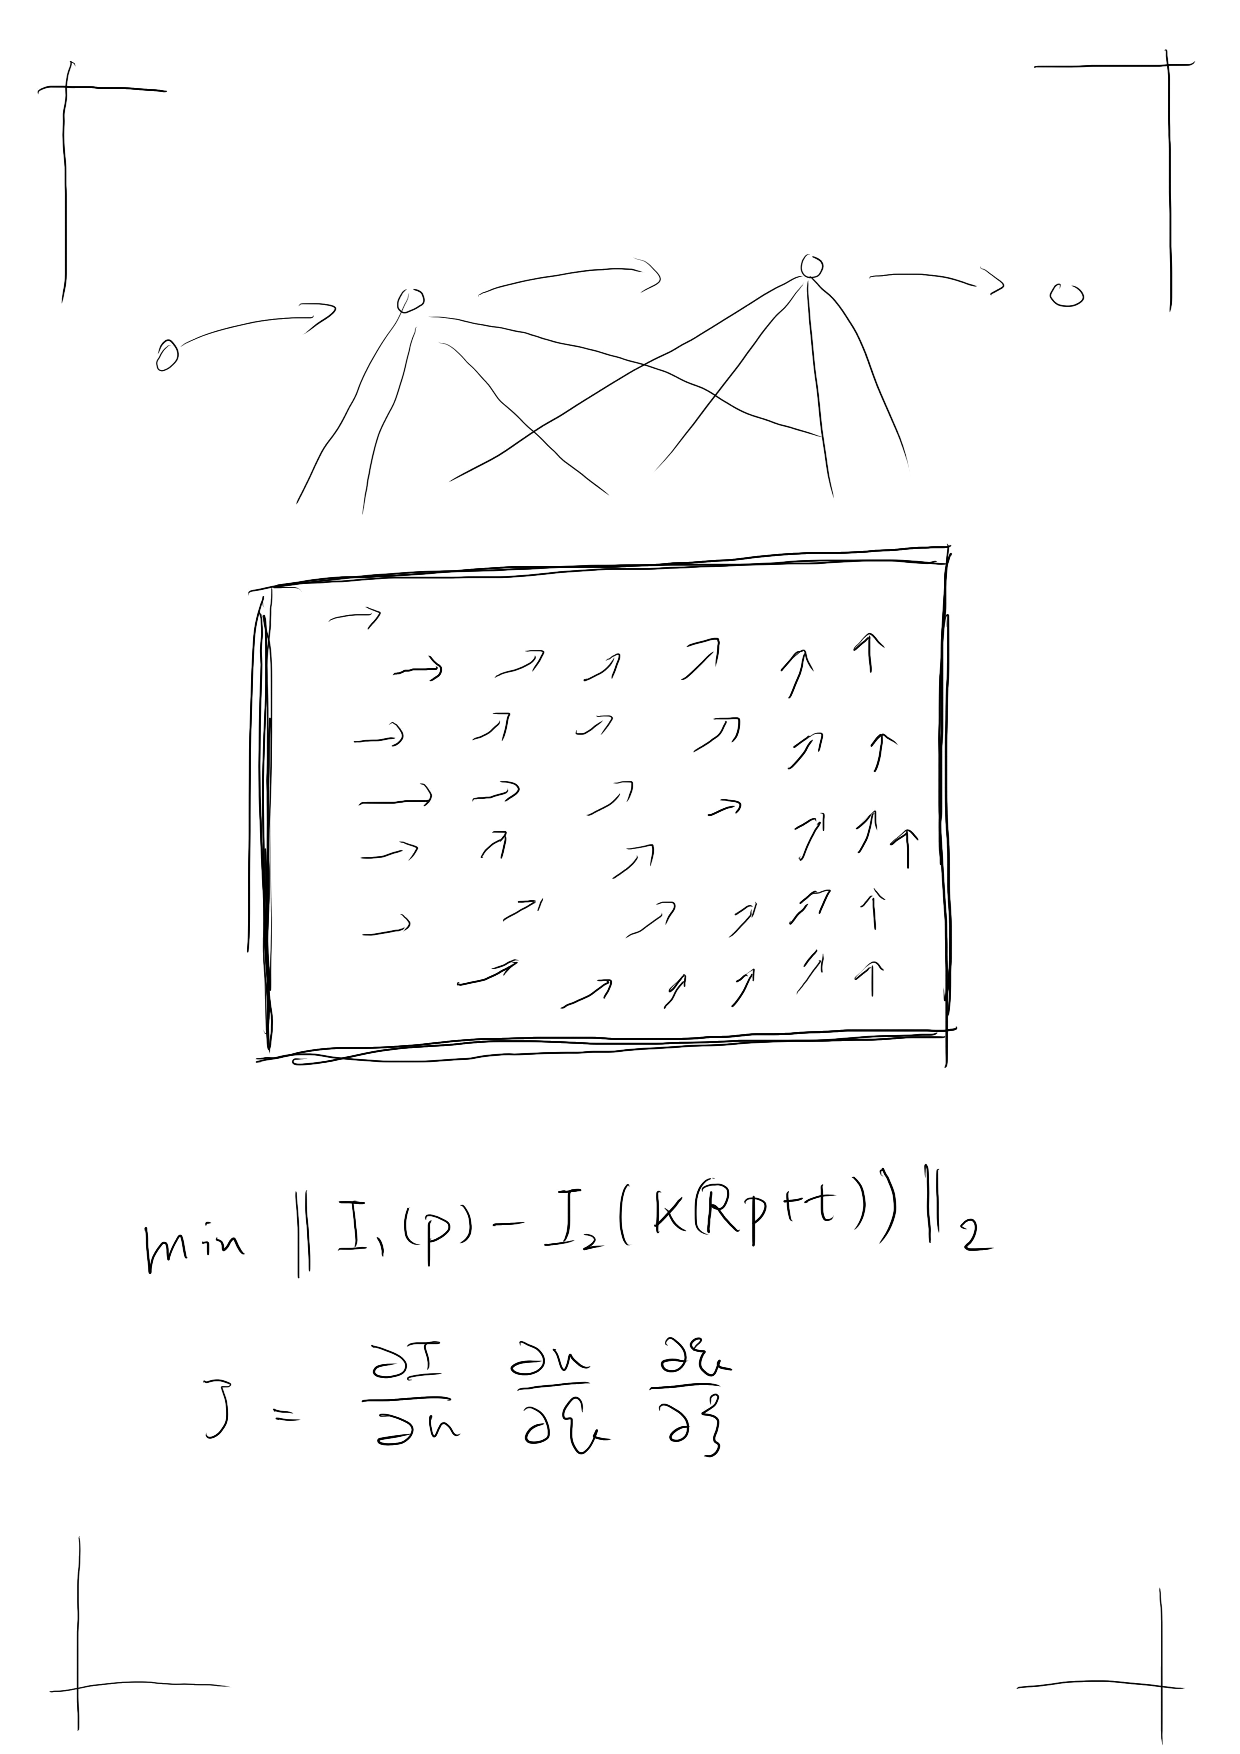
\includepdf{resources/other/ch8.pdf}

\newpage
\section{直接法的引出}
上一讲我们介绍了使用特征点估计相机运动的方法。尽管特征点法在视觉里程计中占据主流地位,但研究者们还是认识到它至少有以下几个缺点:

\begin{enumerate}
	\item 关键点的提取与描述子的计算非常耗时。实践当中,SIFT目前在CPU上是无法实时计算的,而ORB也需要近20ms的计算。如果整个SLAM以30毫秒/帧的速度运行,那么一大半时间都将花在计算特征点上。
	
	\item 使用特征点时,忽略了除特征点以外的所有信息。一幅图像有几十万个像素,而特征点只有几百个。只使用特征点丢弃了大部分\textbf{可能有用的}图像信息。
	
	\item 相机有时会运动到\textbf{特征缺失}的地方,这些地方往往没有明显的纹理信息。例如,有时我们会面对一堵白墙,或者一个空荡荡的走廊。这些场景下特征点数量会明显减少,我们可能找不到足够的匹配点来计算相机运动。 
\end{enumerate}

我们看到使用特征点确实存在一些问题。有没有什么办法能够克服这些缺点呢?我们有以下几种思路:

\begin{itemize}
	\item 保留特征点,但只计算关键点,不计算描述子。同时,使用\textbf{光流法}(Optical Flow)来跟踪特征点的运动。这样可以回避计算和匹配描述子带来的时间,而光流本身的计算时间要小于描述子的计算与匹配。
	\item 只计算关键点,不计算描述子。同时,使用\textbf{直接法}(Direct Method)来计算特征点在下一时刻图像中的位置。这同样可以跳过描述子的计算过程,也省去了光流的计算时间。
\end{itemize}

第一种方法仍然使用特征点,只是把匹配描述子替换成了光流跟踪,估计相机运动时仍使用对极几何、PnP或ICP算法。这依然会要求提取到的关键点具有可区别性,即我们需要提到角点。而在直接法中,我们会根据图像的\textbf{像素灰度信息}同时估计相机运动和点的投影,不要求提取到的点必须为角点。后文将看到,它们甚至可以是随机的选点。

使用特征点法估计相机运动时,我们把特征点看作固定在三维空间的不动点。根据它们在相机中的投影位置,通过\textbf{最小化重投影误差}(Reprojection error)来优化相机运动。在这个过程中,我们需要精确地知道空间点在两个相机中投影后的像素位置——这也就是我们要对特征进行匹配或跟踪的原因。同时,我们也知道,计算、匹配特征需要付出大量的计算量。相对地,在直接法中,我们并不需要知道点与点之间的对应关系,而是通过最小化\textbf{光度误差}(Photometric error)来求得它们。

直接法是本讲介绍的重点。它是为了克服特征点法的上述缺点而存在的。直接法根据像素的亮度信息估计相机的运动,可以完全不用计算关键点和描述子,于是,既避免了特征的计算时间,也避免了特征缺失的情况。只要场景中存在明暗变化(可以是渐变,不形成局部的图像梯度),直接法就能工作。根据使用像素的数量,直接法分为稀疏、稠密和半稠密三种。相比于特征点法只能重构稀疏特征点(稀疏地图),直接法还具有恢复稠密或半稠密结构的能力。

历史上,早期也有对直接法的使用\textsuperscript{\cite{Silveira2008}}。随着一些使用直接法的开源项目的出现(如SVO\textsuperscript{\cite{Forster2014}}、LSD-SLAM\textsuperscript{\cite{Engel2014}}、DSO\textsuperscript{\cite{Engel2016}}等),它们逐渐地走上主流舞台,成为视觉里程计算法中重要的一部分。

\section{2D光流(Optical Flow)}
直接法是从光流演变而来的。它们非常相似,具有相同的假设条件。光流描述了像素在图像中的运动,而直接法则附带着一个相机运动模型。为了说明直接法,我们不妨先来介绍一下光流。

光流是一种描述像素随时间在图像之间运动的方法,如\autoref{fig:LK}~所示。随着时间的流逝,同一个像素会在图像中运动,而我们希望追踪它的运动过程。其中,计算部分像素运动的称为\textbf{稀疏光流},计算所有像素的称为\textbf{稠密光流}。稀疏光流以Lucas-Kanade光流\textsuperscript{\cite{Lucas1981}}为代表,并可以在SLAM中用于跟踪特征点位置。稠密光流以Horn-Schunck光流\textsuperscript{\cite{Horn1981}}为代表。因此,本节主要介绍Lucas-Kanade光流,亦称LK光流。

\begin{figure}[!htp]
	\centering
	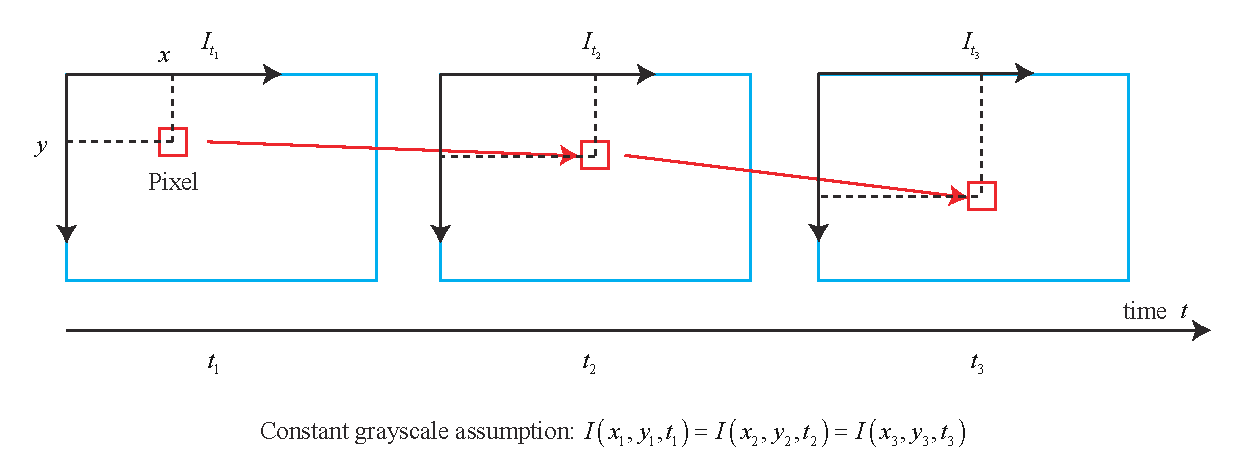
\includegraphics[width=1.0\linewidth]{vo2/opticalFlow}
	\caption{LK光流法示意图。}
	\label{fig:LK}
\end{figure}

\subsection*{Lucas-Kanade光流}
在LK光流中,我们认为来自相机的图像是随时间变化的。图像可以看作时间的函数:$\bm{I}(t)$。那么,一个在$t$时刻,位于$(x,y)$处的像素,它的灰度可以写成
\[
\bm{I}(x,y,t).
\]
这种方式把图像看成了关于位置与时间的函数,它的值域就是图像中像素的灰度。现在考虑某个固定的空间点,它在$t$时刻的像素坐标为$x,y$。由于相机的运动,它的图像坐标将发生变化。我们希望估计这个空间点在其他时刻图像中位置。怎么估计呢?这里要引入光流法的基本假设。

\textbf{灰度不变假设}:同一个空间点的像素灰度值,在各个图像中是固定不变的。

对于$t$时刻位于$(x,y)$处的像素,我们设$t+\mathrm{d}t$时刻它运动到$(x+\mathrm{d}x, y+\mathrm{d}y)$处。由于灰度不变,我们有:
\begin{equation} 
\bm{I}(x+\mathrm{d}x, y+\mathrm{d}y, t+\mathrm{d}t) = \bm{I} (x,y,t).
\end{equation}

注意灰度不变假设是一个很强的假设,实际当中很可能不成立。事实上,由于物体的材质不同,像素会出现高光和阴影部分;有时,相机会自动调整曝光参数,使得图像整体变亮或变暗。这些时候灰度不变假设都是不成立的,因此光流的结果也不一定可靠。然而,从另一方面来说,所有算法都是在一定假设下工作的。如果我们什么假设都不做,就没法设计实用的算法。所以,让我们暂且认为该假设成立,看看如何计算像素的运动。

对左边进行泰勒展开,保留一阶项,得:
\begin{equation}
\bm{I} \left( {x + \mathrm{d}x,y + \mathrm{d}y,t + \mathrm{d}t} \right) \approx \bm{I} \left( {x,y,t} \right) + \frac{{\partial \bm{I} }}{{\partial x}}\mathrm{d}x + \frac{{\partial \bm{I}}}{{\partial y}}\mathrm{d}y + \frac{{\partial \bm{I}}}{{\partial t}}\mathrm{d}t.
\end{equation}

因为我们假设了灰度不变,于是下一个时刻的灰度等于之前的灰度,从而:
\begin{equation}
 \frac{{\partial \bm{I} }}{{\partial x}}\mathrm{d}x + \frac{{\partial \bm{I}}}{{\partial y}}\mathrm{d}y + \frac{{\partial \bm{I}}}{{\partial t}}\mathrm{d}t = 0.
\end{equation}

两边除以$\mathrm{d}t$,得:
\begin{equation}\label{key}
 \frac{{\partial \bm{I} }}{{\partial x}} \frac{\mathrm{d}x}{\mathrm{d}t} + \frac{{\partial \bm{I}}}{{\partial y}} \frac{\mathrm{d}y}{\mathrm{d}t} =- \frac{{\partial \bm{I}}}{{\partial t}}.
\end{equation}

其中$\mathrm{d}x / \mathrm{d}t$为像素在$x$轴上的运动速度,而$\mathrm{d}y/\mathrm{d}t$为$y$轴上的速度,把它们记为$u,v$。同时$\partial \bm{I}/{\partial x}$为图像在该点处$x$方向的梯度,另一项则是在$y$方向的梯度,记为$\bm{I}_x, \bm{I}_y$。把图像灰度对时间的变化量记为$\bm{I}_t$,写成矩阵形式,有:
\begin{equation}
\left[ {\begin{array}{*{20}{c}}
	{{ \bm{I}_x}}&{{ \bm{I}_y}}
	\end{array}} \right]\left[ \begin{array}{l}
u\\
v
\end{array} \right] =  - {\bm{I}_t}.
\end{equation}

我们想计算的是像素的运动$u,v$,但是该式是带有两个变量的一次方程,仅凭它无法计算出$u,v$。因此,必须引入额外的约束来计算$u,v$。在LK光流中,我们假设\textbf{某一个窗口内的像素具有相同的运动}。

考虑一个大小为$w \times w$的窗口,它含有$w^2$数量的像素。由于该窗口内像素具有同样的运动,因此我们共有$w^2$个方程:
\begin{equation}
\left[ {\begin{array}{*{20}{c}}
	{{ \bm{I}_x}}&{{ \bm{I}_y}}
	\end{array}} \right]_k
\left[ \begin{array}{l}
u\\
v
\end{array} \right] =  - {\bm{I}_t}_k, \quad k=1, \ldots, w^2.
\end{equation}

记:
\begin{equation}
\bm{A} = \left[ {\begin{array}{*{20}{c}}
	{{{\left[ {{\bm{I}_x},{\bm{I}_y}} \right]}_1}}\\
	\vdots \\
	{{{\left[ {{\bm{I}_x},{\bm{I}_y}} \right]}_k}}
	\end{array}} \right],\bm{b} = \left[ {\begin{array}{*{20}{c}}
	{{ \bm{I}_{t1}}}\\
	\vdots \\
	{{ \bm{I}_{tk}}}
	\end{array}} \right].
\end{equation}

于是整个方程为
\begin{equation}
\bm{A}\left[ \begin{array}{l}
u\\
v
\end{array} \right] =  - \bm{b}.
\end{equation}

这是一个关于$u,v$的超定线性方程,传统解法是求最小二乘解。最小二乘在很多时候都用到过:
\begin{equation}
{\left[ \begin{array}{l}
	u\\
	v
	\end{array} \right]^*} = -{\left( {{ \bm{A}^\mathrm{T}}\bm{A}} \right)^{ - 1}}{ \bm{A}^\mathrm{T}}\bm{b}.
\end{equation}

这样就得到了像素在图像间的运动速度$u,v$。当$t$取离散的时刻而不是连续时间时,我们可以估计某块像素在若干个图像中出现的位置。由于像素梯度仅在局部有效,所以如果一次迭代不够好,我们会多迭代几次这个方程。在SLAM中,LK光流常被用来跟踪角点的运动,我们不妨通过程序体会一下。

\section{实践:LK光流}
\label{sec:LKFlow}
%\subsection{使用TUM公开数据集}
%下面演示如何用OpenCV提供的光流法来跟踪特征点。与上一节一样,我们准备了若干幅数据集图像,存放在程序目录中的data/文件夹下。它们来自于慕尼黑工业大学(TUM)提供的公开RGB-D数据集\footnote{见\url{http://vision.in.tum.de/data/datasets/rgbd-dataset/download}。}。以后我们就称之为TUM数据集。它含有许多个RGB-D视频,可以作为RGB-D或单目SLAM的实验数据。它还提供了用运动捕捉系统测量的精确轨迹,可以作为标准轨迹以校准SLAM系统。由于该数据集比较大,我们没有放到GitHub上(否则下载代码需要很长时间),请读者自行去数据集主页查找对应的数据。本程序中使用了一部分“freburg1\_desk”数据集中的图像。读者可以在TUM数据集主页找到它的下载链接。或者,也可以直接使用本书在GitHub上提供的部分。
%
%我们的数据位于本章目录的data/下,以压缩包形式提供(data.tar.gz)。由于TUM数据集是从实际环境中采集的,需要解释一下它的数据格式(数据集一般都有自己定义的格式)。在解压后,你将看到以下这些文件:
%
%\begin{enumerate}
%	\item rgb.txt和depth.txt记录了各文件的采集时间和对应的文件名。
%	\item rgb/ 和 depth/目录存放着采集到的PNG格式图像文件。彩色图像为8位3通道,深度图为16位单通道图像。文件名即采集时间。
%	
%	\item groundtruth.txt为外部运动捕捉系统采集到的相机位姿,格式为
%	\[
%	(\mathrm{time}, t_x, t_y, t_z, q_x, q_y, q_z, q_w),
%	\]
%	我们可以把它看成标准轨迹。
%\end{enumerate}
%
%请注意,彩色图、深度图和标准轨迹的采集都是独立的,轨迹的采集频率比图像高很多。在使用数据之前,需要根据采集时间对数据进行一次时间上的对齐,以便对彩色图和深度图进行配对。原则上,我们可以把采集时间相近于一个阈值的数据,看成是一对图像。并把相近时间的位姿,看作是该图像的真实采集位置。TUM提供了一个Python脚本“associate.py”(或使用slambook/tools/associate.py)帮我们完成这件事。请把此文件放到数据集目录下,运行:
%\begin{lstlisting}[language=sh]
%python associate.py rgb.txt depth.txt > associate.txt
%\end{lstlisting}
%
%这段脚本会根据输入的两个文件中的采集时间进行配对,最后输出到文件associate.txt。输出文件含有配对后的两幅图像的时间、文件名信息,可以作为后续处理的来源。此外,TUM数据集还提供了比较估计轨迹与标准轨迹的工具,我们将在用到的地方再进行介绍。
\subsection{使用LK光流}
在实践部分,我们将使用几张示例图像,用OpenCV的光流来追踪上面的特征点。同时,我们也将手动实现一个LK光流,以达到加深理解的效果。我们使用两张来自Euroc数据集的示例图像,在第一张图像中提取角点,然后用光流追踪它们在第二张中的位置。首先我们来使用OpenCV中的LK光流:

\begin{lstlisting}[language=c++,caption=slambook2/ch8/optical_flow.cpp(片段)]
// use opencv's flow for validation
vector<Point2f> pt1, pt2;
for (auto &kp: kp1) pt1.push_back(kp.pt);
vector<uchar> status;
vector<float> error;
cv::calcOpticalFlowPyrLK(img1, img2, pt1, pt2, status, error);
\end{lstlisting}

OpenCV的光流在使用上十分简单,只需调用cv::calcOpticalFlowPyrLK函数,提供前后两张图像以及对应的特征点,即可得到追踪后的点,以及各点的状态、误差。我们可以根据status变量是否为1来确定对应的点是否正确被追踪到。该函数还有一些可选的参数,但是在演示中我们只使用默认参数。我们在此省略其他提特征、画结果的代码,这些在之前的程序中已经展示过了。

\subsection{用高斯牛顿法实现光流}
\subsubsection{单层光流}
光流也可以看成一个优化问题:通过最小化灰度误差,来估计最优的像素偏移。所以,类似于之前实现的各种高斯牛顿法化,我们现在也来实现一个基于高斯牛顿法的光流。

\begin{lstlisting}[language=c++,caption=slambook2/ch8/optical_flow.cpp(片段)]
class OpticalFlowTracker {
public:
	OpticalFlowTracker(
		const Mat &img1_,
		const Mat &img2_,
		const vector<KeyPoint> &kp1_,
		vector<KeyPoint> &kp2_,
		vector<bool> &success_,
		bool inverse_ = true, bool has_initial_ = false) :
		img1(img1_), img2(img2_), kp1(kp1_), kp2(kp2_), success(success_), inverse(inverse_),
		has_initial(has_initial_) {}
	
	void calculateOpticalFlow(const Range &range);

private:
	const Mat &img1;
	const Mat &img2;
	const vector<KeyPoint> &kp1;
	vector<KeyPoint> &kp2;
	vector<bool> &success;
	bool inverse = true;
	bool has_initial = false;
};

void OpticalFlowSingleLevel(
	const Mat &img1,
	const Mat &img2,
	const vector<KeyPoint> &kp1,
	vector<KeyPoint> &kp2,
	vector<bool> &success,
	bool inverse, bool has_initial) {
	kp2.resize(kp1.size());
	success.resize(kp1.size());
	OpticalFlowTracker tracker(img1, img2, kp1, kp2, success, inverse, has_initial);
	parallel_for_(Range(0, kp1.size()),
		std::bind(&OpticalFlowTracker::calculateOpticalFlow, &tracker, placeholders::_1));
}

void OpticalFlowTracker::calculateOpticalFlow(const Range &range) {
	// parameters
	int half_patch_size = 4;
	int iterations = 10;
	for (size_t i = range.start; i < range.end; i++) {
		auto kp = kp1[i];
		double dx = 0, dy = 0; // dx,dy need to be estimated
		if (has_initial) {
			dx = kp2[i].pt.x - kp.pt.x;
			dy = kp2[i].pt.y - kp.pt.y;
		}
		
		double cost = 0, lastCost = 0;
		bool succ = true; // indicate if this point succeeded
		
		// Gauss-Newton iterations
		Eigen::Matrix2d H = Eigen::Matrix2d::Zero();    // hessian
		Eigen::Vector2d b = Eigen::Vector2d::Zero();    // bias
		Eigen::Vector2d J;  // jacobian
		for (int iter = 0; iter < iterations; iter++) {
			if (inverse == false) {
				H = Eigen::Matrix2d::Zero();
				b = Eigen::Vector2d::Zero();
			} else {
				// only reset b
				b = Eigen::Vector2d::Zero();
			}
			
			cost = 0;
			
			// compute cost and jacobian
			for (int x = -half_patch_size; x < half_patch_size; x++)
			for (int y = -half_patch_size; y < half_patch_size; y++) {
				double error = GetPixelValue(img1, kp.pt.x + x, kp.pt.y + y) -
					GetPixelValue(img2, kp.pt.x + x + dx, kp.pt.y + y + dy);;  // Jacobian
				if (inverse == false) {
					J = -1.0 * Eigen::Vector2d(
						0.5 * (GetPixelValue(img2, kp.pt.x + dx + x + 1, kp.pt.y + dy + y) -
							GetPixelValue(img2, kp.pt.x + dx + x - 1, kp.pt.y + dy + y)),
						0.5 * (GetPixelValue(img2, kp.pt.x + dx + x, kp.pt.y + dy + y + 1) -
							GetPixelValue(img2, kp.pt.x + dx + x, kp.pt.y + dy + y - 1))
					);
				} else if (iter == 0) {
					// in inverse mode, J keeps same for all iterations
					// NOTE this J does not change when dx, dy is updated, so we can store it and only compute error
					J = -1.0 * Eigen::Vector2d(
						0.5 * (GetPixelValue(img1, kp.pt.x + x + 1, kp.pt.y + y) -
							GetPixelValue(img1, kp.pt.x + x - 1, kp.pt.y + y)),
						0.5 * (GetPixelValue(img1, kp.pt.x + x, kp.pt.y + y + 1) -
							GetPixelValue(img1, kp.pt.x + x, kp.pt.y + y - 1))
					);
				}
				// compute H, b and set cost;
				b += -error * J;
				cost += error * error;
				if (inverse == false || iter == 0) {
					// also update H
					H += J * J.transpose();
				}
			}
			
			// compute update
			Eigen::Vector2d update = H.ldlt().solve(b);
			
			if (std::isnan(update[0])) {
				// sometimes occurred when we have a black or white patch and H is irreversible
				cout << "update is nan" << endl;
				succ = false;
				break;
			}
			
			if (iter > 0 && cost > lastCost) {
				break;
			}
			
			// update dx, dy
			dx += update[0];
			dy += update[1];
			lastCost = cost;
			succ = true;
			
			if (update.norm() < 1e-2) {
				// converge
				break;
			}
		}
		
		success[i] = succ;
		
		// set kp2
		kp2[i].pt = kp.pt + Point2f(dx, dy);
	}
}
\end{lstlisting}

我们在OpticalFlowSingleLevel函数中实现了单层光流函数,其中调用了cv::parallel\_for\_并行调用OpticalFlowTracker::calculateOpticalFlow,该函数计算指定范围内特征点的光流。这个并行for循环内部是Intel tbb库实现的,我们只需按照其接口,将函数本体定义出来,然后将函数作为std::function对象传递给它即可。

在具体函数实现中(即calculateOpticalFlow),我们求解这样一个问题:
\begin{equation}
\mathop {\min }\limits_{\Delta x,\Delta y} \left\| {{\bm{I}_1}\left( {x,y} \right) - {\bm{I}_2}\left( {x + \Delta x,y + \Delta y} \right)} \right\|_2^2.
\end{equation}
因此,残差为括号内部的部分,对应的雅可比为第二个图像在$x + \Delta x,y + \Delta y$处的梯度。此外,根据文献\cite{Baker2004},这里的梯度也可以用第一个图像的梯度$\bm{I}_1 (x,y)$来代替。这种代替的方法称为\textbf{反向}(Inverse)光流法。在反向光流中,$\bm{I}_1 (x,y)$的梯度是保持不变的,所以我们可以在第一次迭代时保留计算的结果,在后续迭代中使用。当雅可比不变时,$\bm{H}$矩阵不变,每次迭代只需计算残差,这可以节省一部分计算量。

\subsubsection{多层光流}
由于我们把光流写成了优化问题,那么就必须假设优化的初始值靠近最优值,才能在一定程度下保障算法的收敛。于是,如果相机运动较快,两张图像差异较明显,那么单层图像光流法容易达到一个局部极小值。这种情况可以通过引入图像金字塔来改善。

\begin{figure}[!htp]
	\centering
	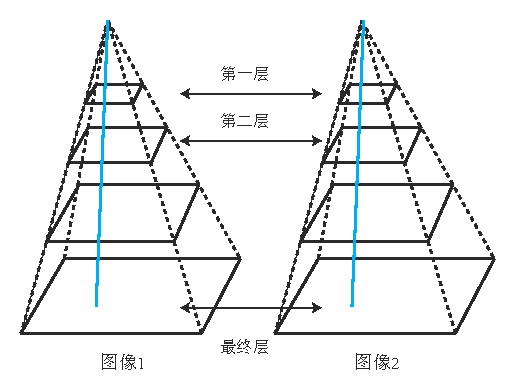
\includegraphics[width=.7\linewidth]{vo2/image-pyramid}
	\caption{图像金字塔和Coarse-to-fine过程。}
	\label{fig:image-pyramid}
\end{figure}

图像金字塔是指对同一个图像进行缩放,得到不同分辨率下的图像,如\autoref{fig:image-pyramid}所示。以原始图像作为金字塔底层,每往上一层,就对下层图像进行一定倍率的缩放,就得到了一个金字塔。然后,在计算光流时,先从顶层的图像开始计算,然后把上一层的追踪结果,作为下一层光流的初始值。由于上层的图像相对粗糙,所以这个过程也称为\textbf{由粗至精}(Coarse-to-fine)的光流,也是实用光流法的通常流程。

由粗至精的好处在于,当原始图像的像素运动较大时,在金字塔顶层的图像看来,运动仍然在一个很小范围内。例如,原始图像的特征点运动了20个像素,很容易由于图像非凸性导致优化困在极小值里。但现在假设有缩放倍率为0.5倍的金字塔,那么往上两层图像里,像素运动就只有5个像素了,这时结果就明显好于直接在原始图像上优化。

我们在程序中实现了多层光流,代码如下:
\begin{lstlisting}[language=c++,caption=slambook2/ch8/optical_flow.cpp(片段)]
void OpticalFlowMultiLevel(
	const Mat &img1,
	const Mat &img2,
	const vector<KeyPoint> &kp1,
	vector<KeyPoint> &kp2,
	vector<bool> &success,
	bool inverse) {
	
	// parameters
	int pyramids = 4;
	double pyramid_scale = 0.5;
	double scales[] = {1.0, 0.5, 0.25, 0.125};
	
	// create pyramids
	vector<Mat> pyr1, pyr2; // image pyramids
	for (int i = 0; i < pyramids; i++) {
		if (i == 0) {
			pyr1.push_back(img1);
			pyr2.push_back(img2);
		} else {
			Mat img1_pyr, img2_pyr;
			cv::resize(pyr1[i - 1], img1_pyr,
			cv::Size(pyr1[i - 1].cols * pyramid_scale, pyr1[i - 1].rows * pyramid_scale));
			cv::resize(pyr2[i - 1], img2_pyr,
			cv::Size(pyr2[i - 1].cols * pyramid_scale, pyr2[i - 1].rows * pyramid_scale));
			pyr1.push_back(img1_pyr);
			pyr2.push_back(img2_pyr);
		}
	}

	// coarse-to-fine LK tracking in pyramids
	vector<KeyPoint> kp1_pyr, kp2_pyr;
	for (auto &kp:kp1) {
		auto kp_top = kp;
		kp_top.pt *= scales[pyramids - 1];
		kp1_pyr.push_back(kp_top);
		kp2_pyr.push_back(kp_top);
	}
	
	for (int level = pyramids - 1; level >= 0; level--) {
		// from coarse to fine
		success.clear();
		OpticalFlowSingleLevel(pyr1[level], pyr2[level], kp1_pyr, kp2_pyr, success, inverse, true);
		
		if (level > 0) {
			for (auto &kp: kp1_pyr)
			kp.pt /= pyramid_scale;
			for (auto &kp: kp2_pyr)
			kp.pt /= pyramid_scale;
		}
	}
	
	for (auto &kp: kp2_pyr)
		kp2.push_back(kp);
}
\end{lstlisting}

这段代码构造了一个四层的,倍率为0.5的金字塔,并调用单层光流函数实现了多层光流。在主函数中,我们分别对两张图像测试了OpenCV的光流、单层光流和多层光流的表现,计算了它们的运行时间:
\begin{lstlisting}[language=sh,caption=终端输入:]
./build/optical_flow
build pyramid time: 0.000150349
track pyr 3 cost time: 0.000304633
track pyr 2 cost time: 0.000392889
track pyr 1 cost time: 0.000382347
track pyr 0 cost time: 0.000375099
optical flow by gauss-newton: 0.00189268
optical flow by opencv: 0.00220134
\end{lstlisting}
从运行时间上来看,多层光流法的耗时和OpenCV大致相当。由于并行化程序在每次运行的表现不尽相同,在读者机器上这些数字不会精确相同。光流的对比图见\autoref{fig:optical-flow-result}。从结果图上看,多层光流与OpenCV的效果相当,单层光流要明显弱于多层光流。

\begin{figure}[!htp]
	\centering
	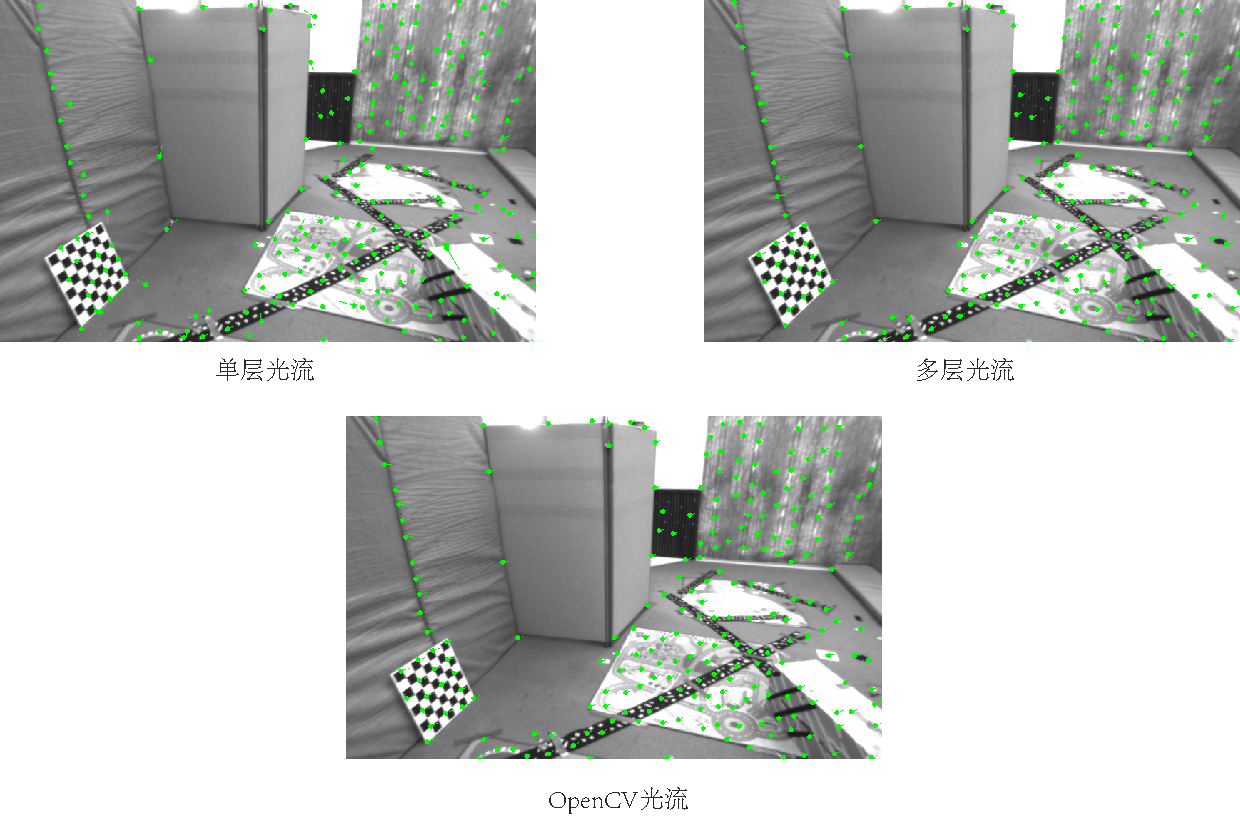
\includegraphics[width=.85\linewidth]{vo2/optical-flow}
	\caption{各种光流的结果对比}
	\label{fig:optical-flow-result}
\end{figure}

\subsection{光流实践小结}
我们看到,LK光流跟踪能够直接得到特征点的对应关系。这个对应关系就像是描述子的匹配,只是光流对图像的连续性和光照稳定性要求更高一些。我们可以通过光流跟踪的特征点,用PnP、ICP或对极几何来估计相机运动,这些方法在上一讲中介绍过,这里不再讨论。

从运行时间上来看,演示实验大约于230个特征点,OpenCV和多层光流需要大约2毫秒完成追踪(我用的CPU是Intel I7-8550U),这实际上是相当快的。如果我们前面使用FAST这样的关键点,那么整个光流计算可以做到5毫秒左右,相比于特征匹配来说算是非常快了。不过,如果角点提的位置不好,光流也容易跟丢或给出错误的结果,这就需要后续算法拥有一定的异常值去除机制,我们留到工程章节再谈。

总而言之,光流法可以加速基于特征点的视觉里程计算法,避免计算和匹配描述子的过程,但要求相机运动较平滑(或采集频率较高)。

\section{直接法(Direct Method)}
接下来,我们来讨论与光流有一定相似性的直接法。与前面内容相似,我们先介绍直接法的原理,然后使用实现一遍直接法。

\subsection{直接法的推导}
在光流中,我们会首先追踪特征点的位置,然后再根据这些位置确定相机的运动。那么,这样一种两步走的方案,很难保证全局的最优性。我们可以问,能不能在后一步中,调整一下前一步的结果呢?比方说,如果我认为相机右转了15度,那么光流能不能以这个15度运动作为初始值的假设,调整光流的计算结果呢?直接法就是遵循这样的思路得到的结果。

如\autoref{fig:directMethod}~所示,考虑某个空间点$P$和两个时刻的相机。$P$的世界坐标为$[X,Y,Z]$,它在两个相机上成像,记像素坐标为$\bm{p}_1, \bm{p}_2$。

\begin{figure}[!htp]
	\centering
	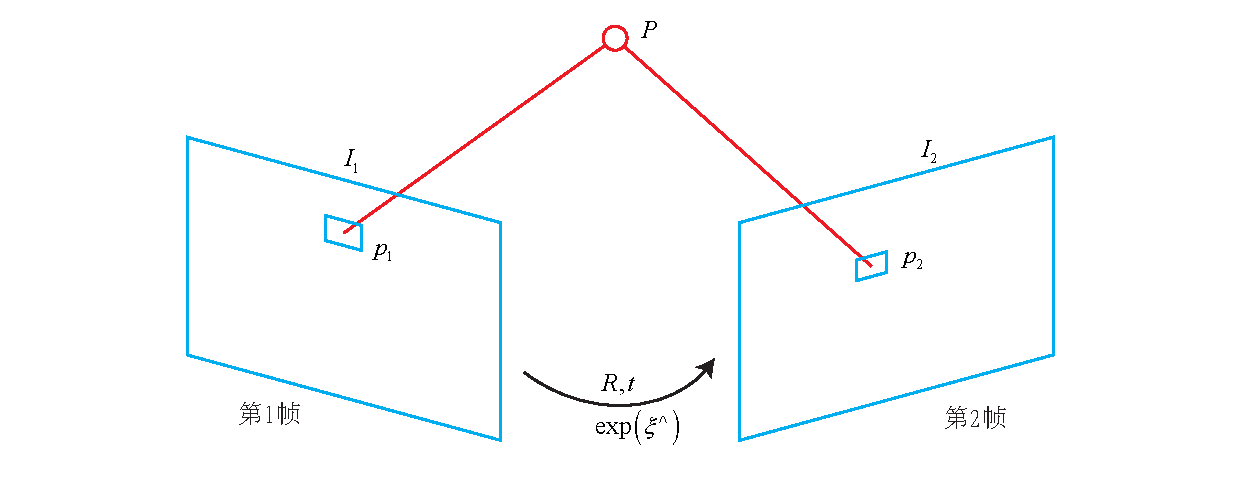
\includegraphics[width=.85\linewidth]{vo2/directMethod}
	\caption{直接法示意图。}
	\label{fig:directMethod}
\end{figure}

我们的目标是求第一个相机到第二个相机的相对位姿变换。我们以第一个相机为参照系,设第二个相机的旋转和平移为$\bm{R}, \bm{t}$(对应李群为$\bm{T}$)。同时,两相机的内参相同,记为$\bm{K}$。为清楚起见,我们列写完整的投影方程:
\begin{align*}
{\bm{p}_1} &= {\left[ \begin{array}{l}
	u\\
	v\\
	1
	\end{array} \right]_1} = \frac{1}{Z_1} \bm{KP}, \\
{\bm{p}_2} &= {\left[ \begin{array}{l}
	u\\
	v\\
	1
	\end{array} \right]_2} = \frac{1}{Z_2} \bm{K}\left( {\bm{RP} +\bm{t}} \right) = \frac{1}{Z_2} \bm{K} \left(\bm{T}  \bm{P} \right)_{1:3}.
\end{align*}
其中$Z_1$是$P$的深度,$Z_2$是$P$在第二个相机坐标系下的深度,也就是$\bm{RP}+\bm{t}$的第3个坐标值。由于$\bm{T}$只能和齐次坐标相乘,所以我们乘完之后要取出前3个元素。这和第\ref{cpt:5}讲的内容是一致的。

回忆特征点法中,由于我们通过匹配描述子知道了$\bm{p}_1, \bm{p}_2$的像素位置,所以可以计算重投影的位置。但在直接法中,由于没有特征匹配,我们无从知道哪一个$\bm{p}_2$与$\bm{p}_1$对应着同一个点。直接法的思路是根据当前相机的位姿估计值来寻找$\bm{p}_2$的位置。但若相机位姿不够好,$\bm{p}_2$的外观和$\bm{p}_1$会有明显差别。于是,为了减小这个差别,我们优化相机的位姿,来寻找与$\bm{p}_1$更相似的$\bm{p}_2$。这同样可以通过解一个优化问题完成,但此时最小化的不是重投影误差,而是\textbf{光度误差}(Photometric Error),也就是$P$的两个像素的亮度误差:
\begin{equation}
e = {\bm{I}_1}\left( {{\bm{p}_1}} \right) - {\bm{I}_2}\left( {{\bm{p}_2}} \right).
\end{equation}

注意这里$e$是一个标量。同样地,优化目标为该误差的二范数,暂时取不加权的形式,为:
\begin{equation}
\mathop {\min }\limits_{\bm{T}}  J\left( \bm{T}  \right) = \|e\|^2.
\end{equation}

能够做这种优化的理由,仍是基于\textbf{灰度不变假设}。我们假设一个空间点在各个视角下成像的灰度是不变的。我们有许多个(比如$N$个)空间点$P_i$,那么,整个相机位姿估计问题变为
\begin{equation}
\mathop {\min }\limits_{\bm{T}}  J\left( \bm{T}  \right) = \sum\limits_{i = 1}^N {e_i^\mathrm{T}{e_i}}, \quad {e_i} = {\bm{I}_1}\left( {{\bm{p}_{1,i}}} \right) - {\bm{I}_2}\left( {{ \bm{p}_{2,i}}} \right).
\end{equation}

注意这里的优化变量是相机位姿$\bm{T}$,而不像光流那样优化各个特征点的运动。为了求解这个优化问题,我们关心误差$e$是如何随着相机位姿$\bm{T}$变化的,需要分析它们的导数关系。因此,定义两个中间变量:
\begin{align*}
\bm{q} &= \bm{T} \bm{P}, \\
\bm{u} &= \frac{1}{{{Z_2}}} \bm{K} \bm{q}.
\end{align*}
这里的$\bm{q}$为$P$在第二个相机坐标系下的坐标,而$\bm{u}$为它的像素坐标。显然$\bm{q}$是$\bm{T}$的函数,$\bm{u}$是$\bm{q}$的函数,从而也是$\bm{T}$的函数。考虑李代数的左扰动模型,利用一阶泰勒展开,因为:
\begin{equation}
e(\bm{T})=\bm{I}_1(\bm{p}_{1})-\bm{I}_2(\bm{u}),
\end{equation}
所以:
\begin{equation}
\frac{\partial e}{\partial \bm{T}} = \frac{{\partial {\bm{I}_2}}}{{\partial \bm{u}}}\frac{{\partial \bm{u}}}{{\partial \bm{q}}}\frac{{\partial \bm{q}}}{{\partial \delta \bm{\xi} }}\delta \bm{\xi},
\end{equation}
其中$\delta \bm{\xi}$为$\bm{T}$的左扰动。我们看到,一阶导数由于链式法则分成了3项,而这3项都是容易计算的:

\begin{enumerate}
	\item $ \partial \bm{I}_2 / \partial \bm{u} $ 为$\bm{u}$处的像素梯度。
	\item $ \partial \bm{u} / \partial \bm{q} $ 为投影方程关于相机坐标系下的三维点的导数。记$\bm{q}=[X,Y,Z]^\mathrm{T}$,根据第$\ref{cpt:7}$讲的推导,导数为
	\begin{equation}
	\frac{{\partial \bm{u}}}{{\partial \bm{q}}} = \left[ {\begin{array}{*{20}{c}}
		{\frac{{\partial u}}{{\partial X}}}&{\frac{{\partial u}}{{\partial Y}}}&{\frac{{\partial u}}{{\partial Z}}}\\
		{\frac{{\partial v}}{{\partial X}}}&{\frac{{\partial v}}{{\partial Y}}}&{\frac{{\partial v}}{{\partial Z}}}
		\end{array}} \right] = \left[ {\begin{array}{*{20}{c}}
		{\frac{{{f_x}}}{{\rm{Z}}}}&0&{ - \frac{{{f_x}X}}{{{Z^2}}}}\\
		0&{\frac{{{f_y}}}{Z}}&{ - \frac{{{f_y}Y}}{{{Z^2}}}}
		\end{array}} \right].
	\end{equation}
	
	\item ${\partial \bm{q}}/{\partial \delta \bm{\xi} }$为变换后的三维点对变换的导数,这在李代数一讲介绍过了:
	\begin{equation}
	\frac{{\partial \bm{q}}}{{\partial \delta \bm{\xi} }} = \left[ { \bm{I}, - {\bm{q}^ \wedge }} \right].
	\end{equation}
\end{enumerate}

在实践中,由于后两项只与三维点$\bm{q}$有关,而与图像无关,我们经常把它合并在一起:
\begin{equation}
\frac{{\partial \bm{u}}}{{\partial \delta \bm{\xi} }} = \left[ {\begin{array}{*{20}{c}}
	{\frac{{{f_x}}}{Z}}&0&{ - \frac{{{f_x}X}}{{{Z^2}}}}&{ - \frac{{{f_x}XY}}{{{Z^2}}}}&{{f_x} + \frac{{{f_x}{X^2}}}{{{Z^2}}}}&{ - \frac{{{f_x}Y}}{Z}}\\
	0&{\frac{{{f_y}}}{Z}}&{ - \frac{{{f_y}Y}}{{{Z^2}}}}&{ - {f_y} - \frac{{{f_y}{Y^2}}}{{{Z^2}}}}&{\frac{{{f_y}XY}}{{{Z^2}}}}&{\frac{{{f_y}X}}{Z}}
	\end{array}} \right].
\end{equation}

这个$2 \times 6$的矩阵在上一讲中也出现过。于是,我们推导出误差相对于李代数的雅可比矩阵:
\begin{equation}
\label{eq:jacobianofDirect}
\bm{J} =  - \frac{{\partial { \bm{I}_2}}}{{\partial \bm{u}}}\frac{{\partial \bm{u}}}{{\partial \delta \bm{\xi} }}.
\end{equation}

对于$N$个点的问题,我们可以用这种方法计算优化问题的雅可比矩阵,然后使用高斯牛顿法或列文伯格—马夸尔特方法计算增量,迭代求解。至此,我们推导了直接法估计相机位姿的整个流程,下面通过程序来演示一下直接法是如何使用的。

\subsection{直接法的讨论}
在上面的推导中,$P$是一个已知位置的空间点,它是怎么来的呢?在RGB-D相机下,我们可以把任意像素反投影到三维空间,然后投影到下一幅图像中。如果是双目,同样可以根据视差来计算像素的深度。如果在单目相机中,这件事情要更为困难,因为我们还须考虑由$P$的深度带来的不确定性。详细的深度估计放到第13讲中讨论。现在我们先来考虑简单的情况,即$P$深度已知的情况。

根据$P$的来源,我们可以把直接法进行分类:
\begin{enumerate}
	\item $P$来自于稀疏关键点,我们称之为稀疏直接法。通常我们使用数百个至上千个关键点,并且像L-K光流那样,假设它周围像素也是不变的。这种稀疏直接法不必计算描述子,并且只使用数百个像素,因此速度最快,但只能计算稀疏的重构。
	\item $P$来自部分像素。我们看到式\eqref{eq:jacobianofDirect}中,如果像素梯度为零,整项雅可比矩阵就为零,不会对计算运动增量有任何贡献。因此,可以考虑只使用带有梯度的像素点,舍弃像素梯度不明显的地方。这称为半稠密(Semi-Dense)的直接法,可以重构一个半稠密结构。
	\item $P$为所有像素,称为稠密直接法。稠密重构需要计算所有像素(一般几十万至几百万个),因此多数不能在现有的CPU上实时计算,需要GPU的加速。但是,如前面所讨论的,像素梯度不明显的点,在运动估计中不会有太大贡献,在重构时也会难以估计位置。
\end{enumerate}

可以看到,从稀疏到稠密重构,都可以用直接法来计算。它们的计算量是逐渐增长的。稀疏方法可以快速地求解相机位姿,而稠密方法可以建立完整地图。具体使用哪种方法,需要视机器人的应用环境而定。特别地,在低端的计算平台上,稀疏直接法可以做到非常快速的效果,适用于实时性较高且计算资源有限的场合\textsuperscript{\cite{Engel2016}}。

\section{实践:直接法}
\subsection{单层直接法}
现在,我们来演示如何使用稀疏的直接法。由于本书不涉及GPU编程,稠密的直接法就省略掉了。同时,为了保持程序简单,我们使用带深度的数据而非单目数据,这样可以省略掉单目的深度恢复部分。基于特征点的深度恢复(即三角化)已经在上一讲介绍过,而基于块匹配的深度恢复将在后面介绍。所以本节我们来考虑双目的稀疏直接法。

由于求解直接法最后等价于求解一个优化问题,因此可以使用g2o或Ceres这些优化库来帮助求解,也可以自己实现高斯牛顿法。和光流类似,直接法也可以分为单层直接法和金字塔式的多层直接法。我们同样先来实现单层直接法,进而拓展到多层。

在单层直接法中,类似于并行的光流,我们也可以并行地计算每个像素点的误差和雅可比,为此我们定义一个求雅可比的类:

\begin{lstlisting}[language=c++,caption=slambook2/ch8/direct_method.cpp(片段)]
/// class for accumulator jacobians in parallel
class JacobianAccumulator {
public:
	JacobianAccumulator(
		const cv::Mat &img1_,
		const cv::Mat &img2_,
		const VecVector2d &px_ref_,
		const vector<double> depth_ref_,
		Sophus::SE3d &T21_) :
	img1(img1_), img2(img2_), px_ref(px_ref_), depth_ref(depth_ref_), T21(T21_) {
		projection = VecVector2d(px_ref.size(), Eigen::Vector2d(0, 0));
	}
	
	/// accumulate jacobians in a range
	void accumulate_jacobian(const cv::Range &range);
	
	/// get hessian matrix
	Matrix6d hessian() const { return H; }
	
	/// get bias
	Vector6d bias() const { return b; }
	
	/// get total cost
	double cost_func() const { return cost; }
	
	/// get projected points
	VecVector2d projected_points() const { return projection; }
	
	/// reset h, b, cost to zero
	void reset() {
		H = Matrix6d::Zero();
		b = Vector6d::Zero();
		cost = 0;
	}
	
private:
	const cv::Mat &img1;
	const cv::Mat &img2;
	const VecVector2d &px_ref;
	const vector<double> depth_ref;
	Sophus::SE3d &T21;
	VecVector2d projection; // projected points
	
	std::mutex hessian_mutex;
	Matrix6d H = Matrix6d::Zero();
	Vector6d b = Vector6d::Zero();
	double cost = 0;
};

void JacobianAccumulator::accumulate_jacobian(const cv::Range &range) {
	
	// parameters
	const int half_patch_size = 1;
	int cnt_good = 0;
	Matrix6d hessian = Matrix6d::Zero();
	Vector6d bias = Vector6d::Zero();
	double cost_tmp = 0;
	
	for (size_t i = range.start; i < range.end; i++) {
		// compute the projection in the second image
		Eigen::Vector3d point_ref =
		depth_ref[i] * Eigen::Vector3d((px_ref[i][0] - cx) / fx, (px_ref[i][1] - cy) / fy, 1);
		Eigen::Vector3d point_cur = T21 * point_ref;
		if (point_cur[2] < 0)   // depth invalid
			continue;
		
		float u = fx * point_cur[0] / point_cur[2] + cx, v = fy * point_cur[1] / point_cur[2] + cy;
		if (u < half_patch_size || u > img2.cols - half_patch_size || v < half_patch_size ||
		v > img2.rows - half_patch_size)
			continue;
		
		projection[i] = Eigen::Vector2d(u, v);
		double X = point_cur[0], Y = point_cur[1], Z = point_cur[2],
		Z2 = Z * Z, Z_inv = 1.0 / Z, Z2_inv = Z_inv * Z_inv;
		cnt_good++;
		
		// and compute error and jacobian
		for (int x = -half_patch_size; x <= half_patch_size; x++)
		for (int y = -half_patch_size; y <= half_patch_size; y++) {
			double error = GetPixelValue(img1, px_ref[i][0] + x, px_ref[i][1] + y) -
				GetPixelValue(img2, u + x, v + y);
			Matrix26d J_pixel_xi;
			Eigen::Vector2d J_img_pixel;
			
			J_pixel_xi(0, 0) = fx * Z_inv;
			J_pixel_xi(0, 1) = 0;
			J_pixel_xi(0, 2) = -fx * X * Z2_inv;
			J_pixel_xi(0, 3) = -fx * X * Y * Z2_inv;
			J_pixel_xi(0, 4) = fx + fx * X * X * Z2_inv;
			J_pixel_xi(0, 5) = -fx * Y * Z_inv;
			
			J_pixel_xi(1, 0) = 0;
			J_pixel_xi(1, 1) = fy * Z_inv;
			J_pixel_xi(1, 2) = -fy * Y * Z2_inv;
			J_pixel_xi(1, 3) = -fy - fy * Y * Y * Z2_inv;
			J_pixel_xi(1, 4) = fy * X * Y * Z2_inv;
			J_pixel_xi(1, 5) = fy * X * Z_inv;
			
			J_img_pixel = Eigen::Vector2d(
				0.5 * (GetPixelValue(img2, u + 1 + x, v + y) - GetPixelValue(img2, u - 1 + x, v + y)),
				0.5 * (GetPixelValue(img2, u + x, v + 1 + y) - GetPixelValue(img2, u + x, v - 1 + y))
			);
			
			// total jacobian
			Vector6d J = -1.0 * (J_img_pixel.transpose() * J_pixel_xi).transpose();
			hessian += J * J.transpose();
			bias += -error * J;
			cost_tmp += error * error;
		}
	}
	
	if (cnt_good) {
		// set hessian, bias and cost
		unique_lock<mutex> lck(hessian_mutex);
		H += hessian;
		b += bias;
		cost += cost_tmp / cnt_good;
	}
}
\end{lstlisting}

在这个类的accumulate\_jacobian函数中,我们对指定范围内的像素点,按照之前的推导计算像素误差和雅可比矩阵,最后加到整体的$\bm{H}$矩阵中。然后,定义一个函数来迭代这个过程:
\begin{lstlisting}[language=c++,caption=slambook2/ch8/direct_method.cpp(片段)]
void DirectPoseEstimationSingleLayer(
	const cv::Mat &img1,
	const cv::Mat &img2,
	const VecVector2d &px_ref,
	const vector<double> depth_ref,
	Sophus::SE3d &T21) {
	const int iterations = 10;
	double cost = 0, lastCost = 0;
	JacobianAccumulator jaco_accu(img1, img2, px_ref, depth_ref, T21);
	
	for (int iter = 0; iter < iterations; iter++) {
		jaco_accu.reset();
		cv::parallel_for_(cv::Range(0, px_ref.size()),
			std::bind(&JacobianAccumulator::accumulate_jacobian, &jaco_accu, std::placeholders::_1));
		Matrix6d H = jaco_accu.hessian();
		Vector6d b = jaco_accu.bias();
		
		// solve update and put it into estimation
		Vector6d update = H.ldlt().solve(b);;
		T21 = Sophus::SE3d::exp(update) * T21;
		cost = jaco_accu.cost_func();
		
		if (std::isnan(update[0])) {
			// sometimes occurred when we have a black or white patch and H is irreversible
			cout << "update is nan" << endl;
			break;
		}
		if (iter > 0 && cost > lastCost) {
			cout << "cost increased: " << cost << ", " << lastCost << endl;
			break;
		}
		if (update.norm() < 1e-3) {
			// converge
			break;
		}
		
		lastCost = cost;
		cout << "iteration: " << iter << ", cost: " << cost << endl;
	}
}
\end{lstlisting}
该函数根据计算的$\bm{H}$和$\bm{b}$,求出对应的位姿更新量,然后更新到当前的估计值上。因为我们在理论部分已经把细节都介绍清楚了,所以这部分代码看起来不会特别困难。

\subsection{多层直接法}
然后,类似于光流,我们再把直接法拓展到金字塔上,用Coarse-to-fine的过程计算相对运动。这部分代码和光流也非常相似:
\begin{lstlisting}[language=c++,caption=slambook2/ch8/direct_method.cpp(片段)]
void DirectPoseEstimationMultiLayer(
	const cv::Mat &img1,
	const cv::Mat &img2,
	const VecVector2d &px_ref,
	const vector<double> depth_ref,
	Sophus::SE3d &T21) {
	// parameters
	int pyramids = 4;
	double pyramid_scale = 0.5;
	double scales[] = {1.0, 0.5, 0.25, 0.125};
	
	// create pyramids
	vector<cv::Mat> pyr1, pyr2; // image pyramids
	for (int i = 0; i < pyramids; i++) {
		if (i == 0) {
			pyr1.push_back(img1);
			pyr2.push_back(img2);
		} else {
			cv::Mat img1_pyr, img2_pyr;
			cv::resize(pyr1[i - 1], img1_pyr,
				cv::Size(pyr1[i - 1].cols * pyramid_scale, pyr1[i - 1].rows * pyramid_scale));
			cv::resize(pyr2[i - 1], img2_pyr,
				cv::Size(pyr2[i - 1].cols * pyramid_scale, pyr2[i - 1].rows * pyramid_scale));
			pyr1.push_back(img1_pyr);
			pyr2.push_back(img2_pyr);
		}
	}
	
	double fxG = fx, fyG = fy, cxG = cx, cyG = cy;  // backup the old values
	for (int level = pyramids - 1; level >= 0; level--) {
		VecVector2d px_ref_pyr; // set the keypoints in this pyramid level
		for (auto &px: px_ref) {
			px_ref_pyr.push_back(scales[level] * px);
		}
		
		// scale fx, fy, cx, cy in different pyramid levels
		fx = fxG * scales[level];
		fy = fyG * scales[level];
		cx = cxG * scales[level];
		cy = cyG * scales[level];
		DirectPoseEstimationSingleLayer(pyr1[level], pyr2[level], px_ref_pyr, depth_ref, T21);
	}	
}
\end{lstlisting}
需要注意的是,因为直接法求雅可比的时候带上了相机的内参,而当金字塔对图像进行缩放时,对应的内参也需要乘以相应的倍率。

\subsection{结果讨论}
最后,我们用一些示例图片来测试直接法的结果。我们使用几张Kitti\textsubscript{\cite{Geiger2013}}自动驾驶数据集的图像。首先,我们读取第一个图像left.png,在对应的视差图disparity.png中,计算每个像素对应的深度,然后对000001.png-000005.png这五张图像,利用直接法计算相机的位姿。为了展示直接法对特征点的不敏感性,我们随机地在第一张图像中选取一些点,不使用任何角点或特征点提取算法,来看看它的结果。
\begin{lstlisting}[language=c++,caption=slambook2/ch8/direct_method.cpp(片段)]
int main(int argc, char **argv) {
	
	cv::Mat left_img = cv::imread(left_file, 0);
	cv::Mat disparity_img = cv::imread(disparity_file, 0);
	
	// let's randomly pick pixels in the first image and generate some 3d points in the first image's frame
	cv::RNG rng;
	int nPoints = 2000;
	int boarder = 20;
	VecVector2d pixels_ref;
	vector<double> depth_ref;
	
	// generate pixels in ref and load depth data
	for (int i = 0; i < nPoints; i++) {
		int x = rng.uniform(boarder, left_img.cols - boarder);  // don't pick pixels close to boarder
		int y = rng.uniform(boarder, left_img.rows - boarder);  // don't pick pixels close to boarder
		int disparity = disparity_img.at<uchar>(y, x);
		double depth = fx * baseline / disparity; // you know this is disparity to depth
		depth_ref.push_back(depth);
		pixels_ref.push_back(Eigen::Vector2d(x, y));
	}
	
	// estimates 01~05.png's pose using this information
	Sophus::SE3d T_cur_ref;
	
	for (int i = 1; i < 6; i++) {  // 1~10
		cv::Mat img = cv::imread((fmt_others % i).str(), 0);
		DirectPoseEstimationMultiLayer(left_img, img, pixels_ref, depth_ref, T_cur_ref);
	}
	return 0;
}
\end{lstlisting}

读者可以尝试在你的机器上运行本段程序,它将输出每个图像的每层金字塔上的追踪点,并输出运行时间。多层直接法的结果如\autoref{fig:direct-experiment}所示。根据程序输出结果,可以看到第五张图像大约是相机往前运动3.8米时的情况。可见,即使我们随机选点,直接法也能够正确追踪大部分的像素,同时估计相机的运动。这中间没有任何的特征提取、匹配或光流的过程。从运行时间上看,在2000个点时,直接法每迭代一层需要1-2毫秒,所以四层金字层约耗时8毫秒左右。相比之下,2000个点的光流耗时大约在十几毫秒左右,还不包括后续的位姿估计。所以,直接法通常相比于传统的特征点和光流要更快一些。

\begin{figure}[!htp]
	\centering
	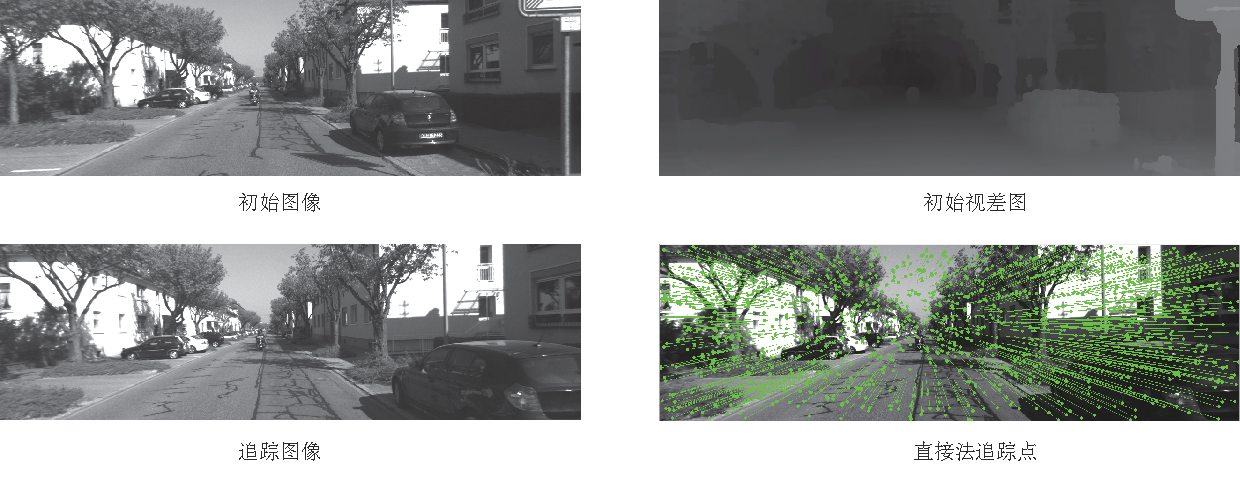
\includegraphics[width=1.0\linewidth]{vo2/direct-experiment}
	\caption{直接法的实验结果。左上:原始图像;右上:原始图像对应的视差图;左下:第五张追踪图像;右下:追踪结果}
	\label{fig:direct-experiment}
\end{figure}

下面我们简单对直接法的迭代过程作一点解释。相比于特征点法,直接法完全依靠优化来求解相机位姿。从式\eqref{eq:jacobianofDirect}中可以看到,像素梯度引导着优化的方向。如果想要得到正确的优化结果,就必须保证\textbf{大部分像素梯度能够把优化引导到正确的方向}。

这是什么意思呢?我们不妨设身处地地扮演一下优化算法。假设对于参考图像,我们测量到一个灰度值为229的像素。并且,由于我们知道它的深度,可以推断出空间点$P$的位置(\autoref{fig:directExperiment}~所示在$I_1$中测量到的灰度)。

\begin{figure}[!htp]
	\centering
	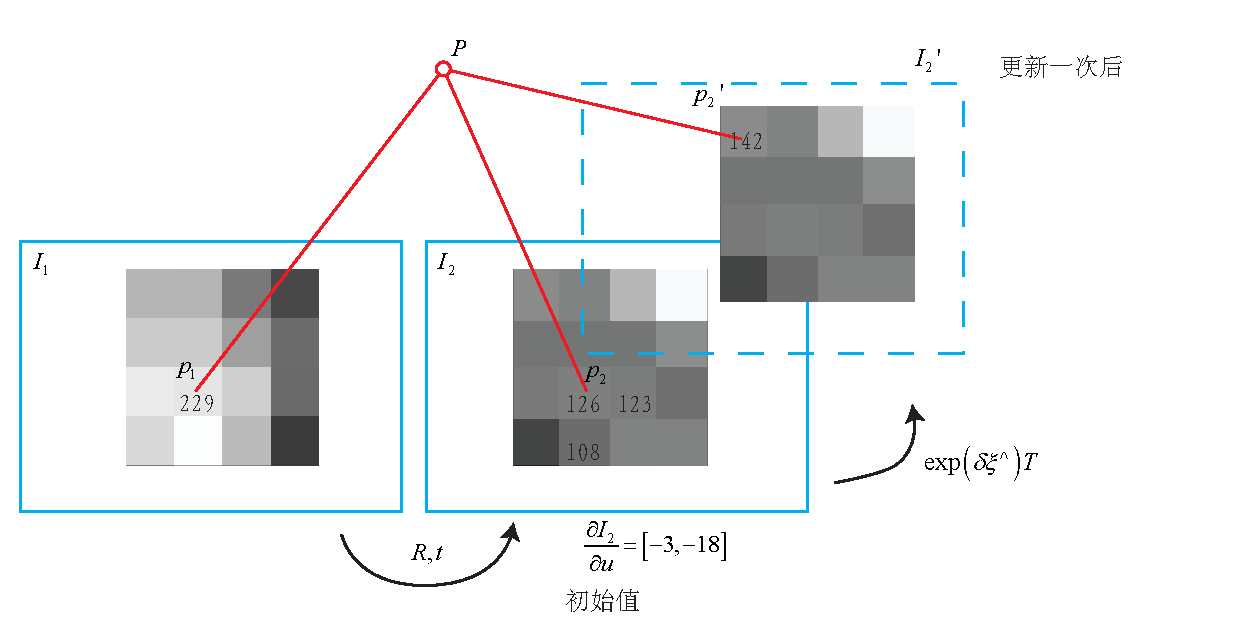
\includegraphics[width=.9\linewidth]{vo2/directExperiment}
	\caption{一次迭代的图形化显示。}
	\label{fig:directExperiment}
\end{figure}

此时我们又得到了一幅新的图像,需要估计它的相机位姿。这个位姿是由一个初值不断地优化迭代得到的。假设我们的初值比较差,在这个初值下,空间点$P$投影后的像素灰度值是126。于是,此像素的误差为$229-126=103$。为了减小这个误差,我们希望\textbf{微调相机的位姿,使像素更亮一些}。

怎么知道往哪里微调像素会更亮呢?这就需要用到局部的像素梯度。我们在图像中发现,沿$u$轴往前走一步,该处的灰度值变成了123,即减去了3。同样地,沿$v$轴往前走一步,灰度值减了18,变成108。在这个像素周围,我们看到梯度是$[-3,-18]$,为了提高亮度,我们会建议优化算法微调相机,使$P$的像往\textbf{左上方}移动。在这个过程中,我们用像素的局部梯度近似了它附近的灰度分布,不过请注意,真实图像并不是光滑的,所以这个梯度在远处就不成立了。

但是,优化算法不能只听这个像素的一面之词,还需要听取其他像素的建议\footnote{这可能是一种不严谨的拟人化说法,不过有助于理解。}。综合听取了许多像素的意见之后,优化算法选择了一个和我们建议的方向偏离不远的地方,计算出一个更新量$\exp ({\bm{\xi}^\wedge } )$。加上更新量后,图像从$I_2$移动到了$I_2'$,像素的投影位置也变到了一个更亮的地方。我们看到,通过这次更新,\textbf{误差变小了}。在理想情况下,我们期望误差会不断下降,最后收敛。

但是实际是不是这样呢?我们是否真的只要沿着梯度方向走,就能走到一个最优值?注意到,直接法的梯度是直接由图像梯度确定的,因此我们必须保证\textbf{沿着图像梯度走时,灰度误差会不断下降}。然而,图像通常是一个很强烈的\textbf{非凸函数},如\autoref{fig:non-convex}~所示。实际当中,如果我们沿着图像梯度前进,很容易由于图像本身的非凸性(或噪声)落进一个局部极小值中,无法继续优化。只有当相机运动很小,图像中的梯度不会有很强的非凸性时,直接法才能成立。

\begin{figure}[!htp]
	\centering
	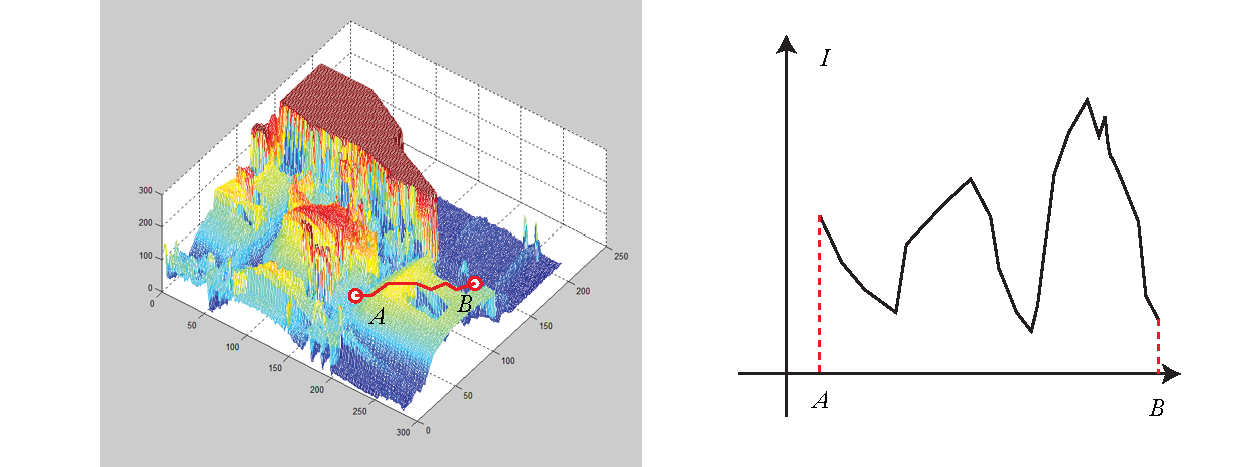
\includegraphics[width=1.0\linewidth]{vo2/nonconvex}
	\caption{一张图像的三维化显示。从图像中的一个点运动到另一个点的路径不见得是“笔直的下坡路”,而需要经常“翻山越岭”。这体现了图像本身的非凸性。}
	\label{fig:non-convex}
\end{figure}

在例程中,我们只计算了单个像素的差异,并且这个差异是由灰度直接相减得到的。然而,单个像素没有什么区分性,周围很可能有好多像素和它的亮度差不多。所以,我们有时会使用小的图像块(patch),并且使用更复杂的差异度量方式,例如归一化相关性(Normalized Cross Correlation,NCC)等。而例程为了简单起见,使用了误差的平方和,以保持与推导的一致性。

\subsection{直接法优缺点总结}
最后,我们总结一下直接法的优缺点。大体上,它的优点如下:

\begin{itemize}
	\item 可以省去计算特征点、描述子的时间。
	\item 只要求有像素梯度即可,不需要特征点。因此,直接法可以在特征缺失的场合下使用。比较极端的例子是只有渐变的一幅图像。它可能无法提取角点类特征,但可以用直接法估计它的运动。在演示实验中,我们看到直接法对随机选取的点亦能正常工作。这一点在实用中非常关键,因为实用场景很有可能没有很多角点可供使用。
	\item 可以构建半稠密乃至稠密的地图,这是特征点法无法做到的。
\end{itemize}

另一方面,它的缺点也很明显:
\begin{itemize}
	\item \textbf{非凸性}。直接法完全依靠梯度搜索,降低目标函数来计算相机位姿。其目标函数中需要取像素点的灰度值,而图像是强烈非凸的函数。这使得优化算法容易进入极小,只在运动很小时直接法才能成功。针对于此,金字塔的引入可以在一定程度上减小非凸性的影响。
	\item \textbf{单个像素没有区分度}。和它像的实在太多了!于是我们要么计算图像块,要么计算复杂的相关性。由于每个像素对改变相机运动的“意见”不一致,只能少数服从多数,以数量代替质量。所以,直接法在选点较少时的表现下降明显,我们通常建议用500个点以上。
	\item \textbf{灰度值不变是很强的假设}。如果相机是自动曝光的,当它调整曝光参数时,会使得图像整体变亮或变暗。光照变化时亦会出现这种情况。特征点法对光照具有一定的容忍性,而直接法由于计算灰度间的差异,整体灰度变化会破坏灰度不变假设,使算法失败。针对这一点,实用的直接法会同时估计相机的曝光参数\cite{Engel2016},以便在曝光时间变化时也能工作。
\end{itemize}

\section*{习题}
\begin{enumerate}
	\item 除了LK光流之外,还有哪些光流方法?它们各有什么特点?
	\item 在本节程序的求图像梯度过程中,我们简单地求了$u+1$和$u-1$的灰度之差除以2,作为$u$方向上的梯度值。这种做法有什么缺点?提示:对于距离较近的特征,变化应该较快;而距离较远的特征在图像中变化较慢,求梯度时能否利用此信息?
	\item 直接法是否能和光流一样,提出“反向法”的概念?即,使用原始图像的梯度代替目标图像的梯度?
	\item[\optional] 使用Ceres或g2o实现稀疏直接法和半稠密直接法。
	\item 相比于RGB-D的直接法,单目直接法往往更加复杂。除了匹配未知之外,像素的距离也是待估计的,我们需要在优化时把像素深度也作为优化变量。阅读文献\cite{Engel2013, Engel2014},你能理解它的原理吗?
\end{enumerate}


